\documentclass[letterpaper, 10pt, conference]{ieeeconf}

\IEEEoverridecommandlockouts                              % This command is only
                                                          % needed if you want to
                                                          % use the \thanks command
\overrideIEEEmargins
% See the \addtolength command later in the file to balance the column lengths^M
% on the last page of the document

% imports
\usepackage{cite}
\usepackage{amssymb}
\usepackage{amsmath}
\usepackage{graphicx}
% \usepackage{qtree}
\usepackage{alltt}
% \usepackage{xfrac}
% bovenstaande wordt nog niet gebruikt, maar is misschien handig in de toekomst
\usepackage[all]{xy}

\usepackage{url}
\urlstyle{same}

\title{\LARGE \bf
Human interface to a humanoid robot}
\author{The authors (Removed for Blind Review)
\thanks{The institute (Removed for Blind Review)}
}

% \author{Duncan Ten Velthuis Auke Wiggers - 6036163\\Steven Laan - 6036031 \\ Supervisor: Roberto Valenti}

\begin{document}
\maketitle
\thispagestyle{empty}
\pagestyle{empty}

\begin{abstract}
This study involves creating a human interface for a humanoid robot by a combination of several interface components. Movements of the human operator are
translated into robot movements with the aid of inverse kinematics. 
This translation cannot be done one-on-one, due tothe difference in build between operator and robot and the limits of the interface components. The robot that is used is the Aldebaran Nao. Interface components that are used are the Xbox 360 Kinect, Vuzix virtual reality glasses and Wii remotes. The robot is controlled through a server/client-connection where the server receives commands and synchronize the commands from the different channels. The result is a humanoid robot which can be controlled in a natural way to handle objects, demonstrated with a Towers of Hanoi task.
\end{abstract}

\section{INTRODUCTION}
The goal of the study is let a human operator control a robot, using its body, i.e.\ without a joystick. The robot mimics the motions of the user, through use depth camera, the Microsoft Kinect. Software that works with the Kinect can extract a wireframe of a human body when someone is in front of the Kinect. This wireframe is then used to find angles of the various joints of the user and map these to the joint angles of the robot through inverse kinematics. Visual information from the robots cameras is sent to virtual reality glasses. These glasses also have a gyroscope which makes it possible for the user to control the head of the robot simply by looking around.

The study will have been successful if the Nao can mimic the users arms and head and if visual information can be seen through the virtual reality glasses. The goal can thus be rephrased as `Controlling a robot using a human interface’.
The system we implemented is a basic version of the human interface: Controlling of robots or other machinery through motion instead of buttons. The Nao is not the best humanoid to use in house-holding tasks, since it`s relatively small and its hands are not meant (and usually not even able) to lift heavy objects. It is easy to bring a Nao out of balance and it is much slower than the average robot on wheels. However, this robot is a humanoid with several joints which can all be controlled from a single platform. Commands for the robot are intuitive and are easily replaced by commands for a different robot. All programs connected to the system will be able to control the robot as long as protocol for the commands is followed. This system is easily universally applicable.

\section{RELATED WORK}

Telepresence lets the user experience a remote environment and act upon
it. One way of reaching this, is raising the situation awareness of the human
operator\cite{Sheridan1992, Goodrich2007}. Using virtual reality glasses enhance the situation awareness is demonstrated before\cite{Goza2004,VanErp2006}. 
The immersion into the virtual reality can be quite complete, as illustrated with the anekdote of \cite{Goza2004} that the operators jerk their feet away when the robot drops something and the motion sickness reported by \cite{VanErp2006}.
Using multiple interface components to control the robot is a prerequisite for \cite{Goodrich2007}, because their Robonaut robot 
has 45 degrees of freedom. The humanoid robot used in this studie, Aldebaran's Nao, has 25 degrees of freedom.

Controlling of a humanoid robot with human movements, including gestures and facial movements is also an active field of research \cite{Suay2011, Broccia2011}. %Asfour2008 is about a humanoid following the head and hands of a human
Suay and Chernova \cite{Suay2011} use specific gestures to start certain behaviors on a Nao robot. One of the behaviors is controlling the gaze direction,
another behaviour is mimicking the movements of the human operator. Those behaviors are not combined, because the depth camera cannot detect 
the gaze direction of the human. In our approach this is solved with the sensors inside the VR glasses. 
Broccia, Lisevu and Scateni \cite{Broccia2011} build a humanoid torso on top of a wheeled platform. The head cannot be turn, so the gaze 
direction is no issue here. The torso of the robot is controlled by mimicking the movements of the human upper body; the wheeled platform
is controlled by gestures of the human lower body. Their method
to determine the angles between the human joints is equivalent with our approach, although they use distances, while our
method uses 3D-vectors.

The Tower of Hanoi puzzle has been used as benchmark for HRI experiments before\cite{Wainer2007,Koenig2010}. 
%Kidd2004 was manipulation of three coloured bloks.
Wainer \textit{et. al.}\cite{Wainer2007} used a wheeled robot to investigate the state of the puzzle and gave instructions to a human
to manipulate the disks. Koenig \textit{et. al.}\cite{Koenig2010} uses the Tower of Hanoi puzzle with a Willows Garage PR2 robot doing the 
manipulation, based on instructions from a human operator. A result of this study is the difference in completion time when the operator
can see the robot motions directly and when the operator can only monitor the movements via the user interface.

% Matari\'{c}  
\section{PLATFORM}
Different hardware components are used, these are listed below. 

\begin{figure}[ht]
\center{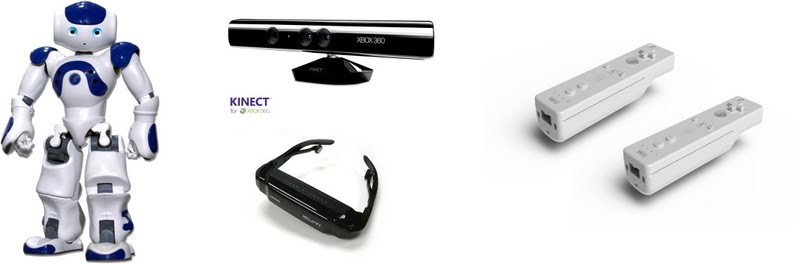
\includegraphics[width = \columnwidth]{Kinect.jpg}}
\label{Components}
\caption{The components our system uses, from left to right and top to bottom: The Aldebaran Nao, the Xbox Kinect, the Vuzix VR glasses and the Wii remotes.}
\end{figure}
\subsection{The robot: The Aldebaran Nao}
The robot that is used is the Aldebaran Nao, Academic version (see Figure~\ref{Components}). The RoboCup edition was used as wel. The difference between the two is that the first has control over its wrists and fingers, which were needed for the mimicking of the hands. The driver software for the Naos was Naoqi 10.10.
\subsection{The Xbox Kinect}
In order to track the body of the human user an Xbox Kinect (see Figure~\ref{Components}) was used. When a user is calibrated the Kinect maps a wireframe to the different joints of the user. Useful output can be derived from this wireframe. The drivers used for the Kinect were in the OpenNI library\footnote{Stable version 1.3, available at \url{http://www.openni.org/}}.
The Kinect is able to track a whole body, but it is only used to track the arms (shoulders and elbows). The output of the Kinect can be a rotation matrix of the joints in respect to the Kinect. This means the Kinect ‘knows’ the orientation of each joint (in respect to its own coordinate system).
The Kinect is also able to estimate the position of all the joints (if they are visible, otherwise it will try to make an educated guess. If even that fails, the position is unknown). This position is relative to the position of the Kinect.

\begin{figure}[htb]
\center{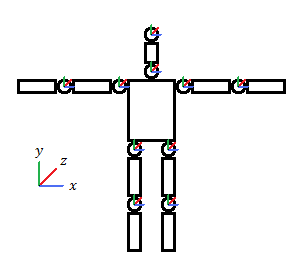
\includegraphics[width = 0.9\columnwidth]{KinectJoints.png}}
\label{KinectJoints}
\caption{The joints as the Kinect sees them. This pose is the zero-orientation, i.e.\ the rotation of all joints is zero. Courtesy NITE project.}
\end{figure}

\subsection{The VR-Glasses}
Because tracking the head is difficult for the Kinect and the orientation of the head is not provided, virtual reality glasses with accelerometers were used to get the orientation of the head. The glasses used are the Vuzix VR920 (see Figure~\ref{Components}). Moreover, images can be sent from the cameras of the Nao to the glasses, enabling the user to see what the robot sees. The SDK from Vuzix was used to retrieve the orientation of the users head.
\subsection{The Wii Remotes}
The Kinect is also bad at determining the lower part of the arms, namely the wrists and hands. In order to be able to mimic the hands another piece of hardware was needed, the Wii Remotes (see Figure~\ref{Components}). The Wii Remote, or informally Wiimote, has several buttons and a built-in accelerometer. The orientation of the hands can be derived from this. It is also possible to use buttons on the remote to control the Nao (for example, open or close hands). It’s also possible to initiate other sequences such as walking or bending the knees.
The software we used for the Wiimotes is `WiiYourself!’ version 1.15.
\section{DESIGN ISSUES}
The task was divided into several subtasks. These subtasks could all be solved independently.
\subsection{Mimicking}
One of the main challenges is the mimicking of the joints by the Nao. Firstly, the context of this task will be explained in more detail, then, the tried approaches are described.
\subsubsection{The task}
Each pose the user makes involves angles for the different joints of the user. These angles can be found using the Kinect and the gyrometer in the VR glasses. The problem is that the Nao does not only have slightly less joints than a human, the reach is also different. For example: while humans have three degrees of freedom in their shoulder (i.e. we can change yaw, pitch and roll), the Nao only has two degrees of freedom (roll and pitch). The problem is that we have to calculate for each pose the angles for the different joints of the Nao; this problem is more generally known as inverse kinematics.
\subsubsection{Approach}
Several approaches are studied, although three approaches were studied in detail. 
%So they will be explained in the order we tried to implement them.
\\
\noindent{\textbf{Euler Angles}}\\
The first thing we thought of was to calculate the Euler angles from the rotation matrix we got from the Kinect. Because the rotation matrices from the Kinect are in respect to the coordinate system of the Kinect itself, we first had to rotate back, in order to make all rotations in respect to the Nao. After we did this transformation we had all rotation matrices of the joints, in the coordinate system of the Nao. Now we could calculate the Euler angles from the rotation matrix. 
%However, this is easier said than done. (?) 
As it turns out, there are always multiple solutions to the problem, i.e. one rotation matrix can be obtained by several Euler angle combinations. In the worst case there are infinitely many solutions, this situation is referred to as a gimbal lock\cite{Shoemake1985}. Luckily, there are several solutions to this problem\cite{euler}. Unfortunately, the gimbal lock isn’t the only problem.
Another problem is that the Nao does not have the same joints as humans do. Therefore a rotation that is quite easy for a human might be impossible for the Nao. This expresses itself for example in the rotation matrix for the shoulder ($s\theta$ and $c\theta$ are abbreviations of $\sin\theta$ and $\cos\theta$ respectively):
\begin{equation}
\label{eq:rotation_matrix}
\begin{bmatrix}
c\theta_1 & -s\theta_1& 0\\
s\theta_1 & c\theta_1 & 0\\
0 & 0 & 1\\
\end{bmatrix}
\begin{bmatrix}
c\theta_2 & 0 & -s\theta_2\\
0 &1&0\\
s\theta_2 & 0 & c\theta_2\\
\end{bmatrix}
=
\begin{bmatrix}
c\theta_1 c\theta_2 & -s\theta_1 & -s\theta_2 c\theta_1\\
s\theta_1 c\theta_2 & c\theta_1 & -s\theta_1 s\theta_2\\
s\theta_2 & 0 & c\theta_2\\
\end{bmatrix}
\end{equation}

The human shoulder is a ball-and-socket joint with three degrees of freedom\cite{Woodson1992}, while the Nao has a swing-and-twist joint with only two degrees of freedom. As you can see in equation~\ref{eq:rotation_matrix}, the Nao can not perform any rotation which is defined by a rotation matrix where the element $R_{32}$ is larger than 0.
As we couldn't find an easy way to solve this problem, we tried another approach.\\\\
\noindent{\textbf{`Forward backward'}}\\
The ‘forward backward’ approach, as we call it, also uses rotation matrices only quite a different way. The idea is that we calculate the position of the end effector (i.e. the hands) and then let the Nao solve the inverse kinematics using its built-in function. The name 'forward backward' is derived from how we calculate the angles: First we use rotation matrices to calculate the hands position (starting at the shoulders position). Then the inverse kinematics calculates the shoulders angles using the hands position. So we go forward from the shoulder to the hand and then backwards from the hand to the shoulder.
This method did work, however since its only the end-effectors position that is mimicked, the pose of the rest of the arm is quite arbitrary. Therefore we looked for another approach.\\\\
\noindent{\textbf{Trigonometry/dotproduct}}\\
The method we’re currently using does not involve rotation matrices. Basically we retrieve the positions of the joints, calculate vectors from them and then use the dot product to get the angle. This approach will be explained in more detail in Section~\ref{sec:architecture}.
\subsection{Realtime datatransfer to/from Nao}
The Kinect and the VR glasses both have to send data to the Nao for it to mimic the user. This has to be done as fast as possible so the Nao can immediately change the angles of its joints.
\subsubsection{The task}
At first we though of using .ini or .txt files to store data locally and then send commands to the Nao based on this data. However, our supervisor suggested we'd use a TCP connection. Through this connection, information can be sent from server to client or vice versa.
The benefit of using this format is that we are solving two problems at a time: The two programming languages that are used to control the Nao (Python) and simultaneously get data from the glasses and Kinect (C++) do not have a direct correspondence but both can handle strings. Limiting the messages to string format does not only keep messages relatively small but also makes it possible to send any message from one program to another, given the right protocol.
\subsubsection{Approach}
A program in C++ that reads data from the gyroscope in the VR glasses calculates the corresponding angle for the Nao’s neck joints, which are then sent to it in the format $<$Jointname$> <$Angle$>$. The same goes for the program that reads data from the Kinect. Depending on the number of connections, other data is appended to the first incoming string, which is then decomposed in the python program that also started the server. First, it is checked if the given angle is possible for the current joint (if the angle is in range of the Nao’s joint) and if that is true, the Nao’s joint is set in that angle. The higher the frequency at which data is sent, the more fluent the Nao’s movements are.
\subsection{Leg control}
Control of the legs of the robot makes it possible to do simple tasks, such as walking around or reaching the ground by bending the knees.
\subsubsection{The task}
Using the Kinect to control the legs seemed to be an impossible task due to balance issues. The Nao has less degrees of freedom and the weight/length-ratio of the limbs is fundamentally different from that of humans. Another problem is that humans make use of momentum and falling during walking and maintaining balance. The Nao can not do this without being at risk of damaging itself. Although the Nao has two built-in gyroscopes, it is hard to predict the consequences of certain motions without a working simulation. Real-time simulation of motions before performing them is simply not possible for every command the clients send.
\subsubsection{Approach}
We tried two different approaches, with varying results.

\noindent{\textbf{Gesture}} \\
The first idea was to control the legs through gestures. Our signal for walking in the direction of the head was pointing forward with the right arm. Since the head is steered by the glasses, Nao walks in the direction the user looks. A benefit of this approach is that the user always sees where the Nao is going. However, accidental activation is possible. When picking up something in front of the Nao, it can occur that the arms need to be stretched, thus involuntarily satisfying the walking condition. It is also possible that due to strong arm movements and a shifted center of gravity the Nao loses balance, especially while walking.

\noindent{\textbf{Wiimote}} \\
A slightly better approach would be to use an external device. Apart from making it possible to mimic hands and wrists and opening/closing the hands, there are several buttons on the Wii remote that can be used to steer the Nao. Movements such as walking or bending the knees are useful when wanting to pick something up. A downside is that the use of the remotes does not contribute to the idea of a human interface, since it involves button use. The standard protocol also has to be changed, since the Nao’s walking movement is steered by a different function entirely. Our protocol has a simple addition of the name of the button followed by a boolean (e.g. LBButton 1 means that the B-button on the left Wii remote is pressed). The server program checks if such a message is sent and if so, executes the corresponding action.

\section{SOLUTION ARCHITECTURE}
\label{sec:architecture}
The TCP server that runs on the Nao is the core of the system (see figure 2). It can connect to a large number of clients which can all send data as long as the protocol for messages is followed. The messages should always be strings so there is no limit to the possible programming languages, as long as a connection to the server can be made. Duplicate messages are not a problem either, since the program only executes the first command in a message containing duplicate (and thus possibly contradicting) joints and angles. The only constraint is that the buffer for the messages is not infinitely big, a message from a client can, in the current program, not be larger than 4096 bytes. The slowest client determines how fast the Nao is able to execute given commands, since the server waits for one message from every client before executing the commands.

\begin{figure}[h]
\label{TCP}
\center
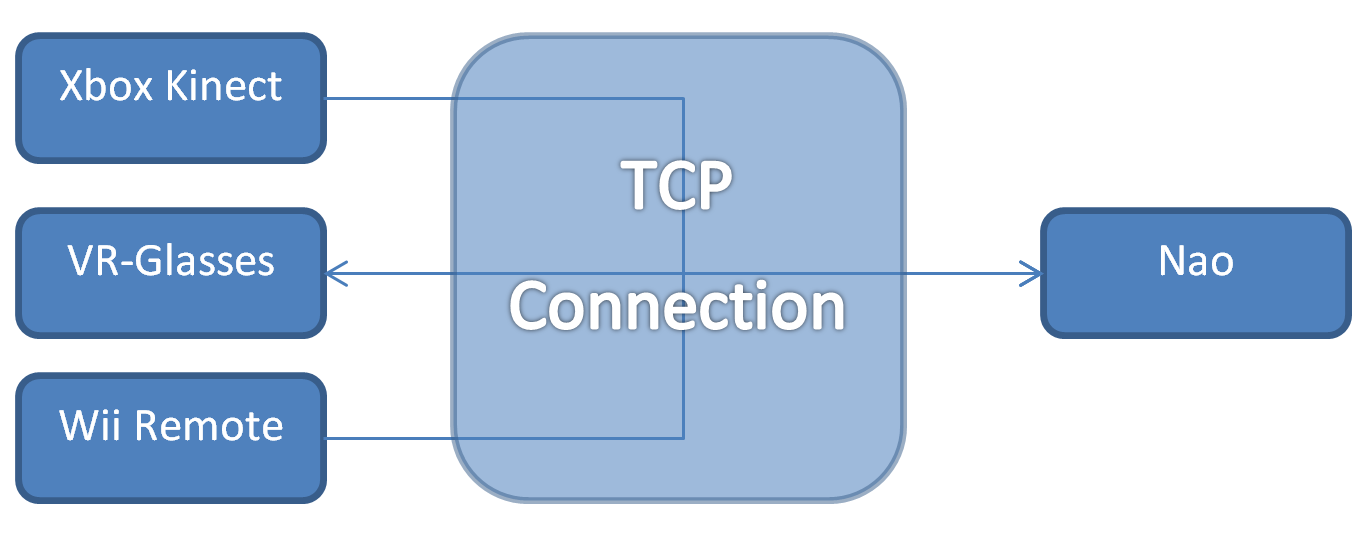
\includegraphics[width = \columnwidth]{figure.png}
\caption{A visual representation of the TCP Connection. All hardware devices send data to the Nao.}
\end{figure}
After initiating the program with the number of connections as input for the start-funtion, clients can connect to the TCP server. Once all three interface components have connected, the Nao will start executing commands from the clients.
The first client we implemented is a program collecting data from the Xbox Kinect. It calculates the angles for the joints of the Nao that correspond to the angles of the users body. This is done through positions of joints involved in that angle. From these positions vectors are calculated. Using the dot product of the two vectors, we can determine the angle between the two.
To illustrate our approach we will give an example. We want to calculate the roll of the right shoulder (see figure 3). Thus we take the positions of the right elbow($p_{E}$), the right hip($p_{H}$) and the right shoulder($p_{S}$) in order to calculate $\angle p_{E}p_{S}p_{H}$.
\begin{figure}
\label{ShoulderRoll}
\center{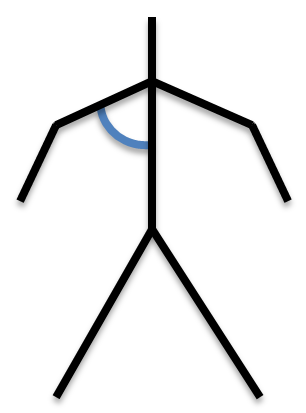
\includegraphics[width = 3.2cm]{StickFigure.png}}
\caption{A stick figure showing the shoulder roll in the Nao}
\end{figure}
We could use normal trigonometry to solve this, because we know all the points in space and thus we can easily calculate the angles. Instead we use the dot product of vectors. This is because for some joints we cannot create a nice triangle, simply because there are not always three joints which perfectly lie in the plane. For example, the elbow yaw cannot be calculated in a triangular fashion. The elbow yaw is the joint that makes you able to turn you lower arm around the axis of your upper arm. So if we wanted to create a triangle that calculates the elbow yaw, we would need the positions of the elbow, the hand and another joint in that plane that is perpendicular to the upper arms axis. There is no such joint, therefore we can’t calculate the angle via trigonometry. Our solution to this problem is that we use vectors, which do not have to have a common point in order to calculate the angle between them. For instance, for the elbow roll we use the vector pointing from the shoulder to the hip and the vector pointing from the elbow to the hand. If we calculate the dot product between the two, we can easily determine the angle (where $\theta$ is the angle between the two vectors):
$$ \vec{a} \cdot \vec{b} = ||\vec{a}|| ||\vec{b}|| \cos{\theta}$$
The second client collects data from the gyroscope in the Vuzix virtual reality glasses. This data is used to determine two angles, a yaw and pitch, for the head of the Nao (the Nao does not have a neck joint for the roll). It also acts as visual input for the user, acting as a second screen for the computer it connects to.
To create this visual input, we use Choreographe, a program by Aldebaran robotics. The benefit of this program is that it can simultaneously show the camera images and the pose of the Nao in simulation. The latter because the real Nao’s body is not visible to users with the glasses on.

\begin{figure}[ht]
\center{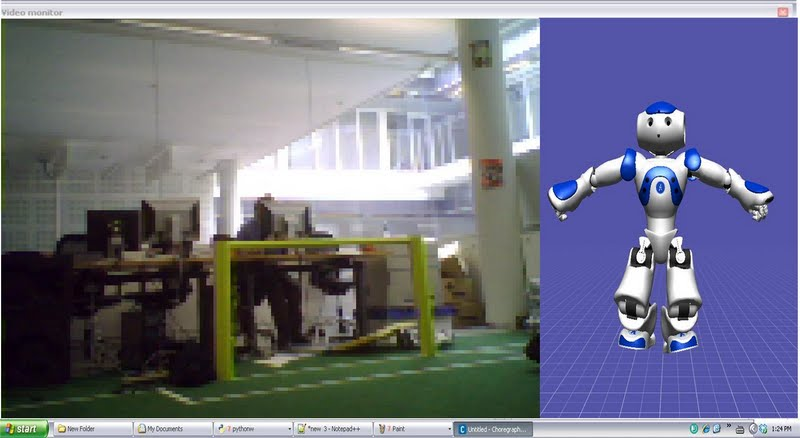
\includegraphics[width = \columnwidth]{images.jpg}}
\label{Choreographe}
\caption{The image, as seen through the virtual reality glasses.}
\end{figure}


\bibliographystyle{IEEEtran}
\section{RESULTS}
We’ve enabled the use of several components to control the Nao.
\subsection{Our results}
With the components we’re currently using (the Xbox Kinect, the Vuzix virtual reality glasses, the Wii remotes, the Aldebaran Nao and Choreograph), the program gives the user a camera view and the pose of the Nao in simulation through the glasses. The Nao itself will mimic the users upper body which is made possible through use of the Kinect and Wiimotes, though this can only be seen in simulation if the user is wearing the VR glasses. Gestures or buttons on the Wii remotes activate walking of the Nao. This enables the user to execute simple remote operations, such as lifting a box or pushing a button. It should be noted that calibration of the VR glasses is needed before use of the system with all it’s current components.


\begin{figure}[ht]
\center{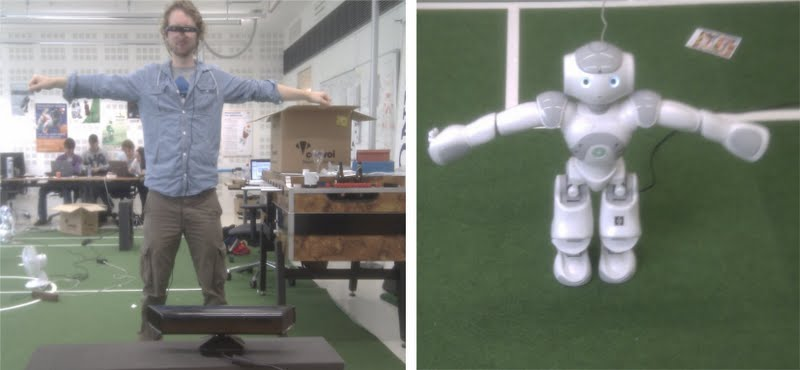
\includegraphics[width = \columnwidth]{Duncan.jpg}}
\label{Duncan}
\caption{An example of the system when using the VR glasses and Kinect.}
\end{figure}

\subsection{Use of this system}
The user starts by initiating the server and client programs. The user then puts on the Vuzix virtual reality glasses, holds the Wii remotes and stands in front of the Xbox Kinect in the calibration pose. When calibration is complete, the server program will start receiving commands from the clients. The client program that controls data transfer from Kinect to Nao sends commands for the upper body. The client reading values from the VR glasses’ gyroscope sends commands for the Nao’s neck joints. The client sending data from the Wii remotes controls the lower body and enables closing and opening of the hands. 
The Nao thus starts mimicking the user as soon as commands are sent. If a single client program stops, all clients and the server program will stop functioning correctly. Once the server has stopped, clients will stop sending data. 
An example of the system in action can be seen in figure 5 and 6.

\subsection{General use}
The system we implemented allows a human user to control humanoid robots through body motions. It does not require the user to lift the legs or walk, only the upper body is mimicked. Requirements for use are perhaps a few hours of practice but no knowledge of robotics is needed. It is therefore applicable in any area. A few examples of possible use are teleoperation in dangerous area’s (e.g.\ after natural disasters or warzones), house-holding tasks but also industrial processes. The human interface makes it relatively easy to learn the robot a new task since it can simply mimic the user executing the task.

\section{CONCLUSION}
The result of this study is the creation of a human interface to a humanoid robot. This could only be done by solving several issues: maintaining balance, the coupling of human kinematics with the humanoid kinematics and synchronizing the different interface components controlling the robot. Balancing the robot is still an issue because of the differences between human and Nao (humans behave fundamentally different in walking and balancing tasks). This problem was not solved, instead, time was spent on implementing a different method for controlling the Nao's legs.

The control system, consisting of one server program and a theoretically infinite number of interface clients (3 clients were chosen in this case because 3 interface components were needed to control all relevant degrees of freedom of the robot), allows smooth teleoperation of the Nao. The server program is exclusively designed for the Aldebaran Nao but this can easily be altered to an equivalent humanoid robot, as long as the control functions are intuitive (e.g. for the Nao setAngles sets angles for given joints, openHand opens the given hand).
While searching for information about the used components, it was clear that there were several students and freelancers who had attempted similar approaches \cite{freiburg} \cite{veltrop}, though this is the first study which uses VR glasses for gaze control.

\bibliography{IEEEabrv,references,bib}

\end{document}
